\documentclass[xcolor=table]{beamer}

\definecolor{light-gray}{gray}{0.8}
\definecolor{light-light-gray}{gray}{0.9}

\beamertemplatenavigationsymbolsempty

\title{Notes on the CAD-Compatible Conversion\\of Multi-Sided Surfaces}
\author{P\'eter Salvi$^\dagger$, Tam\'as V\'arady$^\dagger$, Alyn Rockwood$^\ddagger$}
\institute{$^\dagger$ Budapest University of Technology and Economics\\
           $^\ddagger$ Boulder Graphics LLC, USA}
\date{CAD'20, July 6--8, 2020}

\begin{document}

\begin{frame}
  \titlepage
\end{frame}

\begin{frame}
  \frametitle{Outline}
  \begin{columns}
    \column{0.5\textwidth}
    \tableofcontents
    \column{0.5\textwidth}
    \centering
    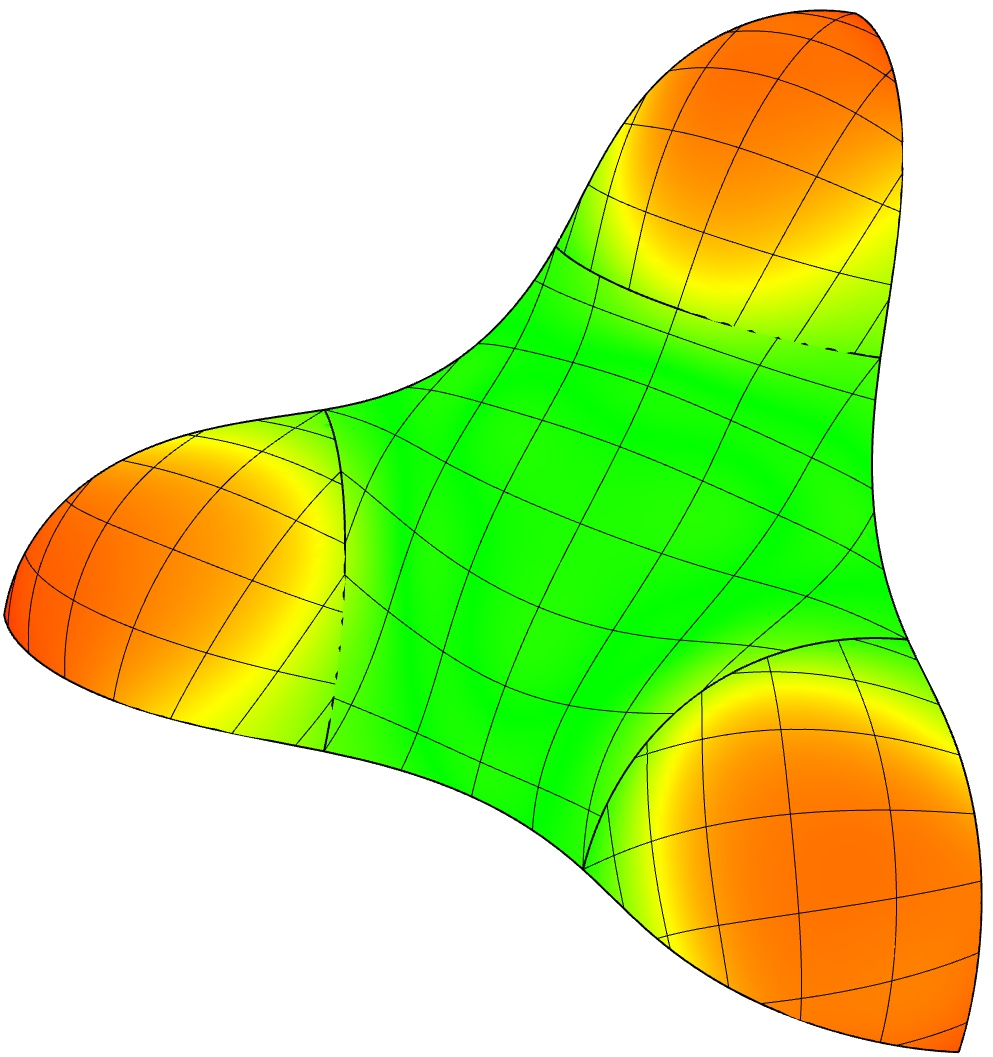
\includegraphics[width=.8\textwidth]{images/trebol3-mean-iso.jpg}
  \end{columns}
\end{frame}

\section{Motivation}

\begin{frame}
  \frametitle{Motivation}
  \begin{columns}
    \column{0.5\textwidth}
    \begin{itemize}
    \item Multi-sided surfaces
    \item Trimming
      \begin{itemize}
      \item Only approximate $C^0$
      \end{itemize}
    \item Splitting
      \begin{itemize}
      \item Reduced continuity\\in the interior
      \end{itemize}
    \item Natively multi-sided patches
      \begin{itemize}
      \item Intuitive controls
      \item Not CAD-compatible
      \end{itemize}
    \item Conversion to NURBS?
    \end{itemize}
    \column{0.5\textwidth}
    \centering
    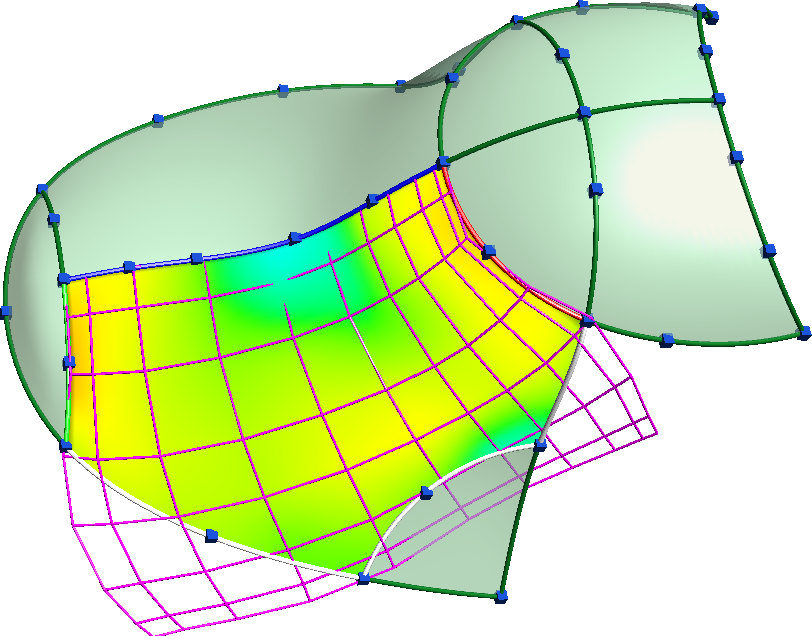
\includegraphics[height=.4\textheight]{images/slides/trim.png}\\
    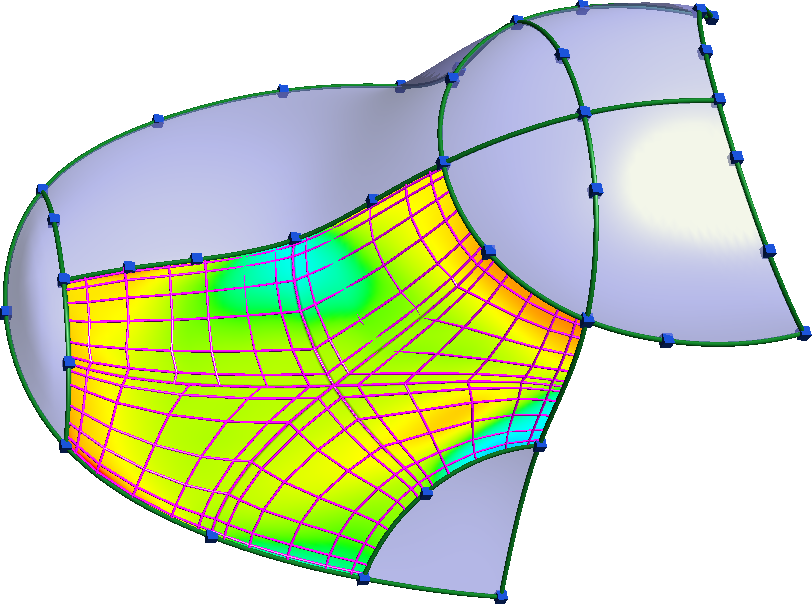
\includegraphics[height=.4\textheight]{images/slides/split.png}
  \end{columns}
\end{frame}

\begin{frame}
  \frametitle{Plan}
  \begin{itemize}
  \item Four multi-sided schemes
    \begin{enumerate}
    \item S-patch
    \item Warren's patch
    \item Kato's patch
    \item Charrot--Gregory patch
    \end{enumerate}
  \item Rational tensor product B\'ezier form
  \item Problems \& workarounds
  \end{itemize}
  \vfill
  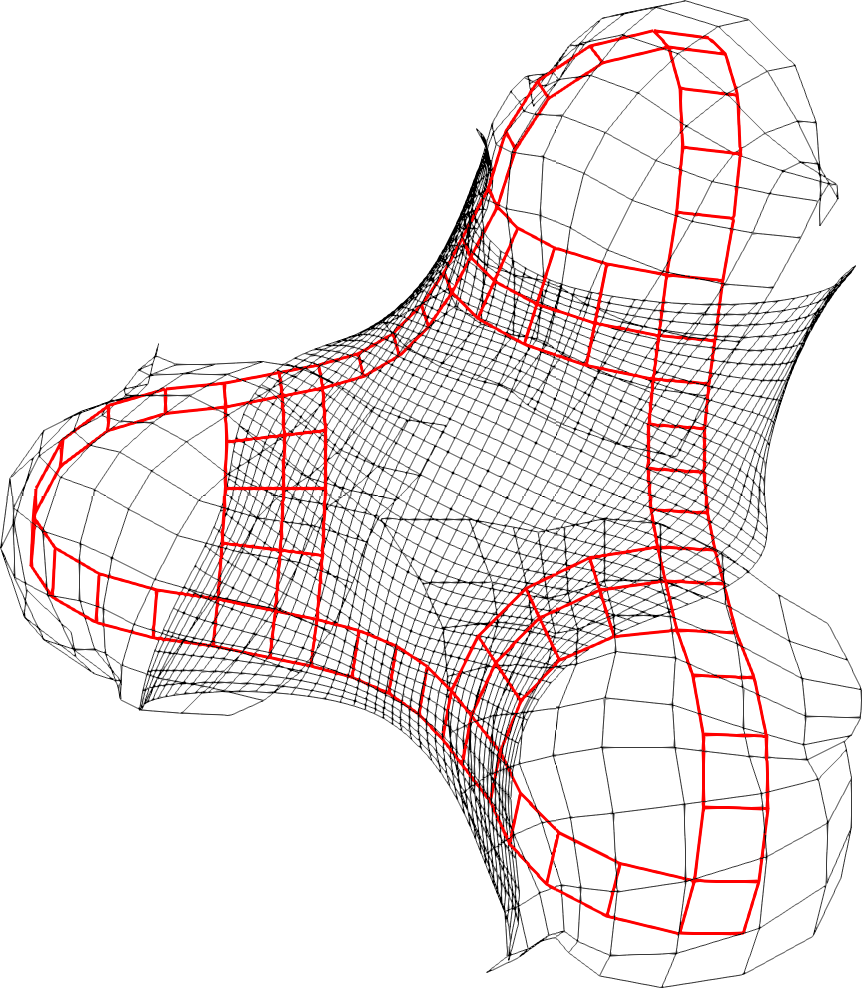
\includegraphics[width=.22\textwidth]{images/trebol3-cnet.png}
  \hfill
  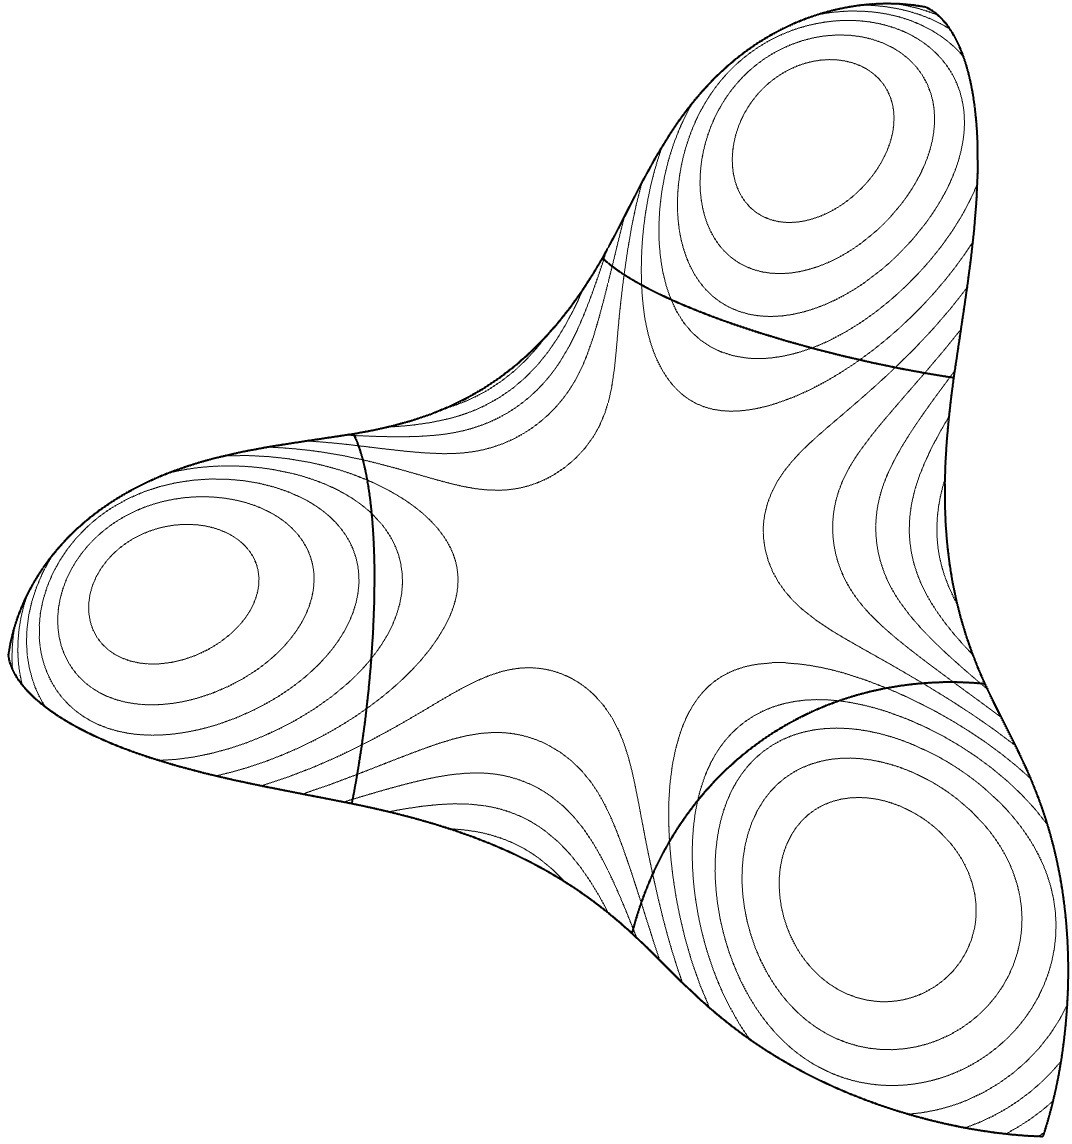
\includegraphics[width=.24\textwidth]{images/trebol3-contour.jpg}
  \hfill
  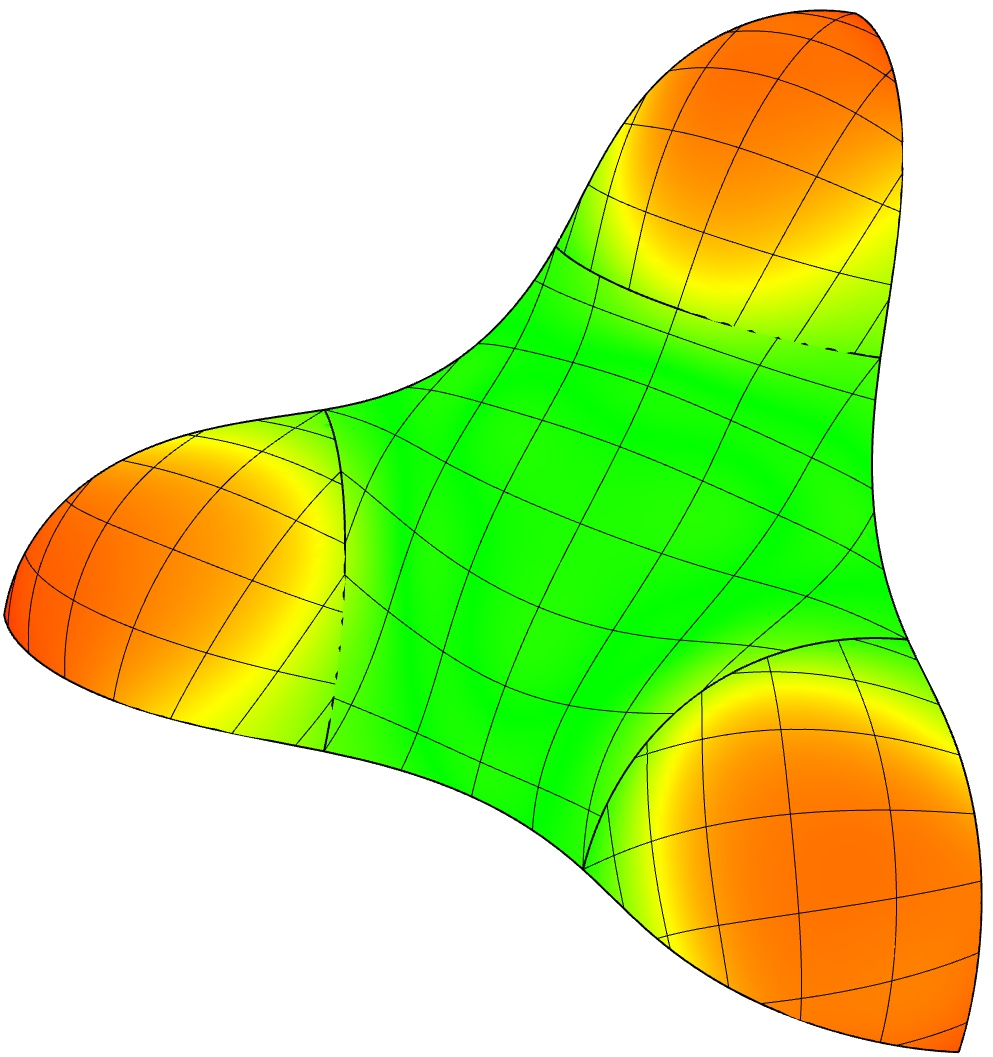
\includegraphics[width=.24\textwidth]{images/trebol3-mean-iso.jpg}
  \hfill
  
\includegraphics[width=.24\textwidth]{images/trebol3-zebra.jpg}
\end{frame}

\AtBeginSection[]{
 \begin{frame}
   \frametitle{Outline}
   \tableofcontents[currentsection]
 \end{frame}
}

\section{S-patches}
\subsection{Patch equation}

\begin{frame}
  \frametitle{S-patch}
  \[
  S(\mathbf{\lambda})=\sum_{\mathbf{s}}P_\mathbf{s}\cdot B_\mathbf{s}^d(\mathbf{\lambda})
  =\sum_{\mathbf{s}}P_\mathbf{s}\cdot {d\choose\mathbf{s}}\cdot\prod_{i=1}^n\lambda_i^{s_i}
  \]
  \begin{itemize}
  \item $n$: \# of sides
  \item $d$: depth (\# of de Casteljau steps)
  \item $\mathbf{s}$: indices; $\mathbf{s}=(s_1,\dots,s_n)$, $|\mathbf{s}|=d$
  \item $P_\mathbf{s}$: control points
  \item $\mathbf{\lambda}$: generalized barycentric coordinates;
    $\mathbf{\lambda}=(\lambda_1,\dots,\lambda_n)$
  \item Regular polygonal domain
  \end{itemize}
  \vfill
  \centering
  Polynomial except for $\mathbf{\lambda}$
\end{frame}

\subsection{$G^1$ frames}

\begin{frame}
  \frametitle{Control structure}
  \begin{itemize}
  \item Too many control points for interactive use
  \item $n=d=5\Rightarrow126$ (cf.~quintic tensor product B\'ezier $\Rightarrow36$)
  \item $G^1$ frame: positional- and tangent plane boundary constraints
  \item Two-step surface generation
    \begin{enumerate}
    \item Boundary interpolation ($d=$ degree\,$+3$)
    \item Interior (global system)
    \end{enumerate}
  \end{itemize}
  \vfill
  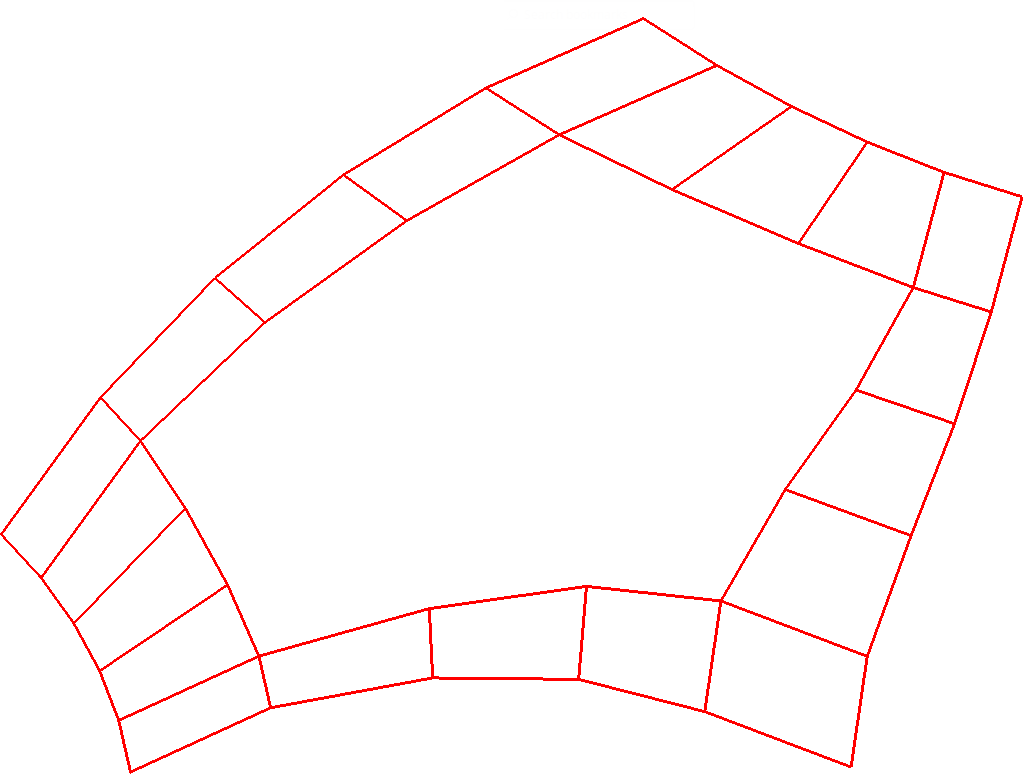
\includegraphics[width = 0.31\textwidth]{images/5-5-bezier-ribbon.png}
  \hfill
  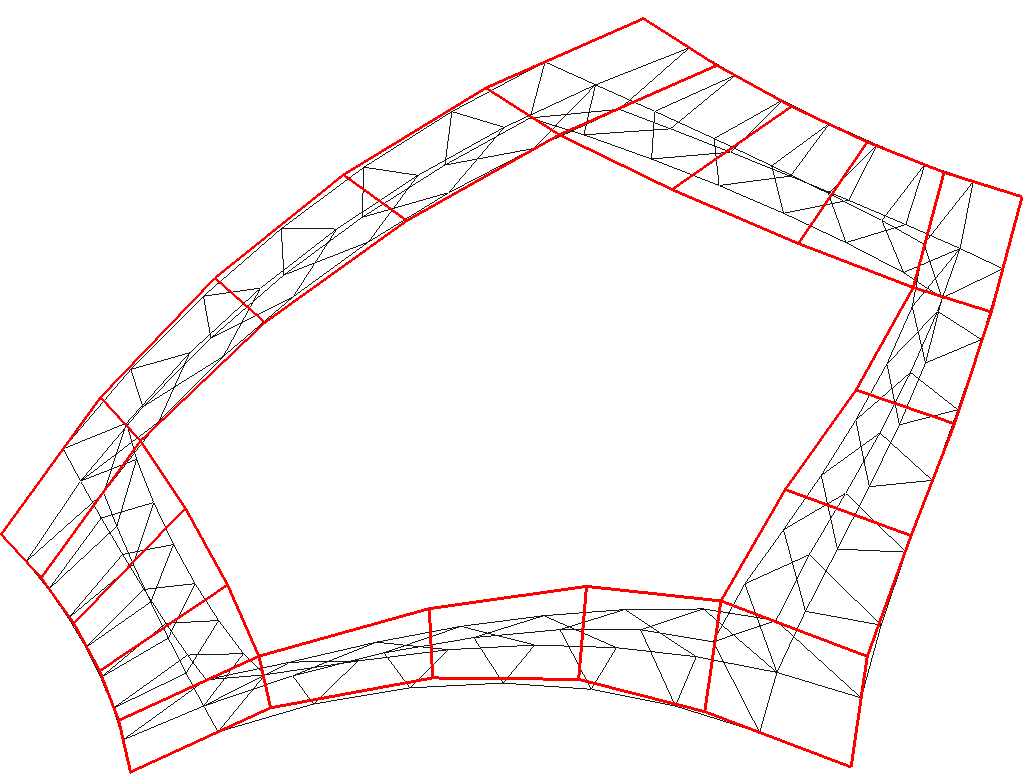
\includegraphics[width = 0.31\textwidth]{images/5-5-cnet-ribbon.png}
  \hfill
  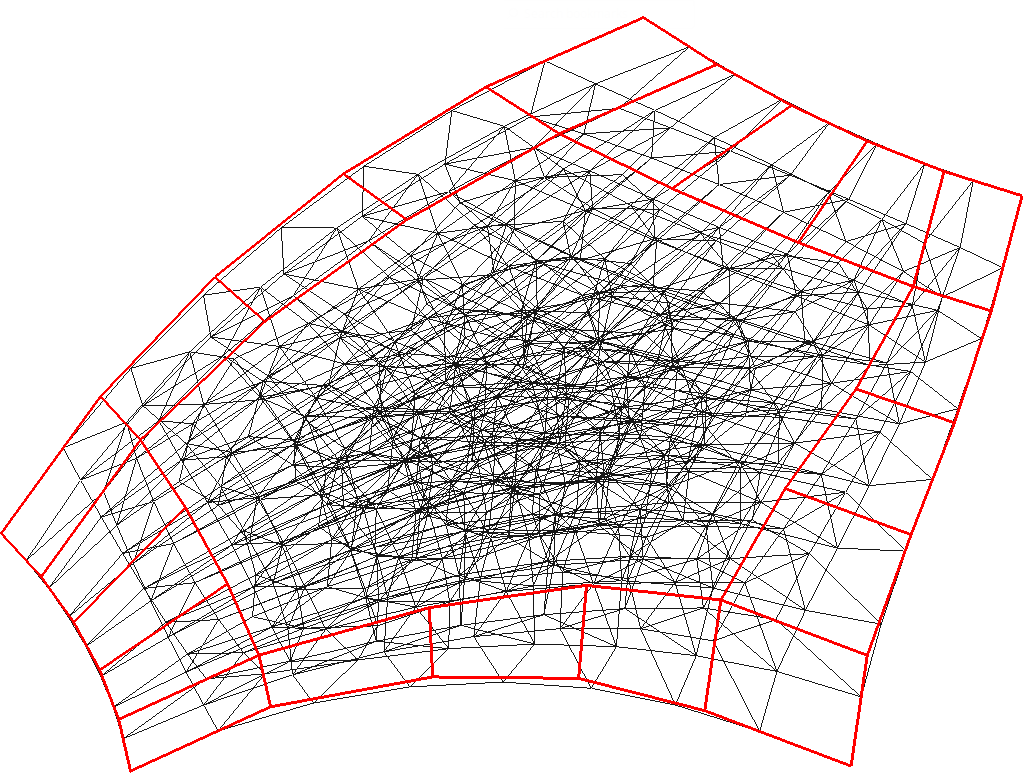
\includegraphics[width = 0.31\textwidth]{images/5-5-cnet-full.png}
\end{frame}

\subsection{Parameters by line equations}

\begin{frame}
  \frametitle{Conversion to rational B\'ezier form}
  \begin{center}
    Problem: $\{\lambda_i\}$ $\rightarrow$ rational polynomials in $(u,v)$
  \end{center}
  \vfill
  \begin{columns}
    \column{0.65\textwidth}
    \begin{itemize}
    \item {[Loop \& DeRose]}
      \begin{itemize}
      \item Composition of B\'ezier simplexes
      \item High complexity $\Rightarrow$ slow
      \end{itemize}
    \item Wachspress coordinates
      \begin{itemize}
      \item Rational function of the distances $h_k$ from the domain edges
      \end{itemize}
    \item Implicit line equations
      \begin{itemize}
      \item $L(u,v)=Au+Bv+C=0$
      \item Linear signed distance functions
      \end{itemize}
    \item $h_k:=L_k$
      \begin{itemize}
      \item Normalized to 1 on adjacent vertices
      \end{itemize}
    \end{itemize}
    \column{0.35\textwidth}
    \centering
    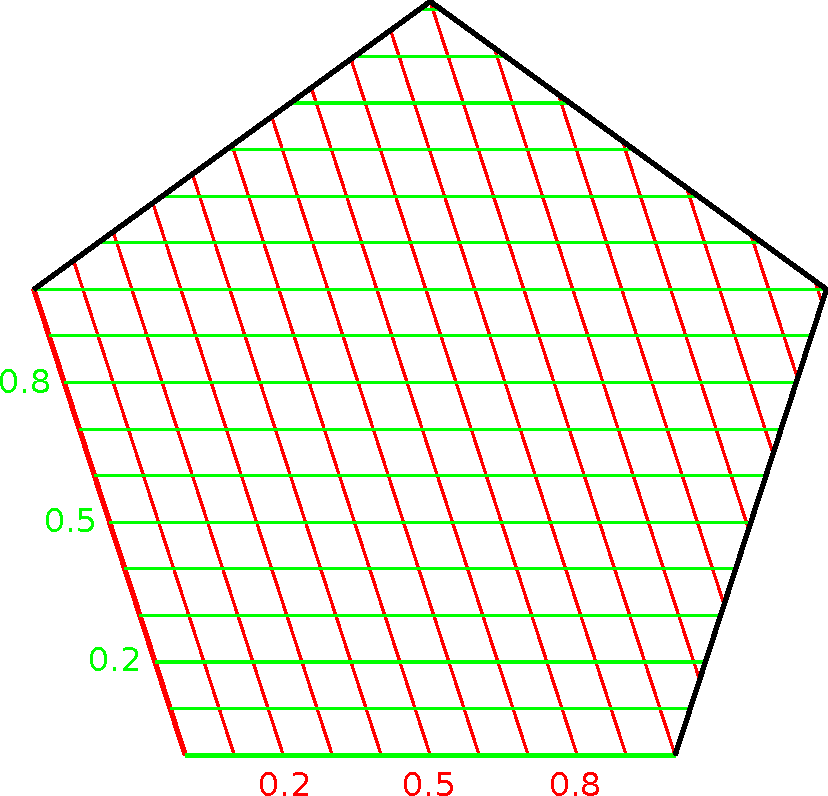
\includegraphics[width=\textwidth]{images/h-params.pdf}
  \end{columns}
\end{frame}

\section{Other multi-sided patches}
\subsection{Warren's patch}

\begin{frame}
  \frametitle{Warren's patch}
  \begin{columns}
    \column{0.65\textwidth}
    \begin{itemize}
    \item Cuts off B\'ezier triangle corners
    \item $0/0$ \emph{base points} -- not standard!
    \item Simple $G^1$ interpolation
    \item Simple polynomial conversion
      \begin{align*}
        \lambda_1&=(1-u)v, & \lambda_2&=uv, & \lambda_3&=1-v
      \end{align*}
    \item Only 5- and 6-sided
    \item Not all degree configurations allowed
    \item Distorted parameters
      \begin{itemize}
        \item Domain corners $\approx$ 3D edges
      \end{itemize}
    \end{itemize}
    \column{0.35\textwidth}
    \centering
    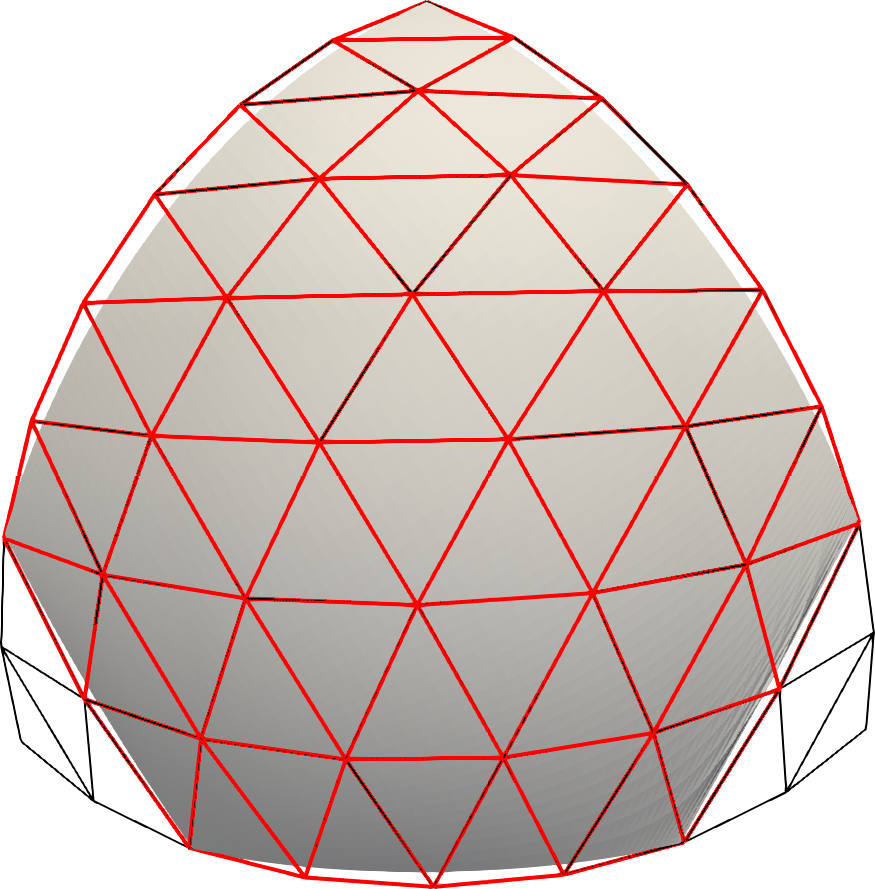
\includegraphics[height=.35\textheight]{images/warren-cnet.png}\\
    \vspace{1.5em}
    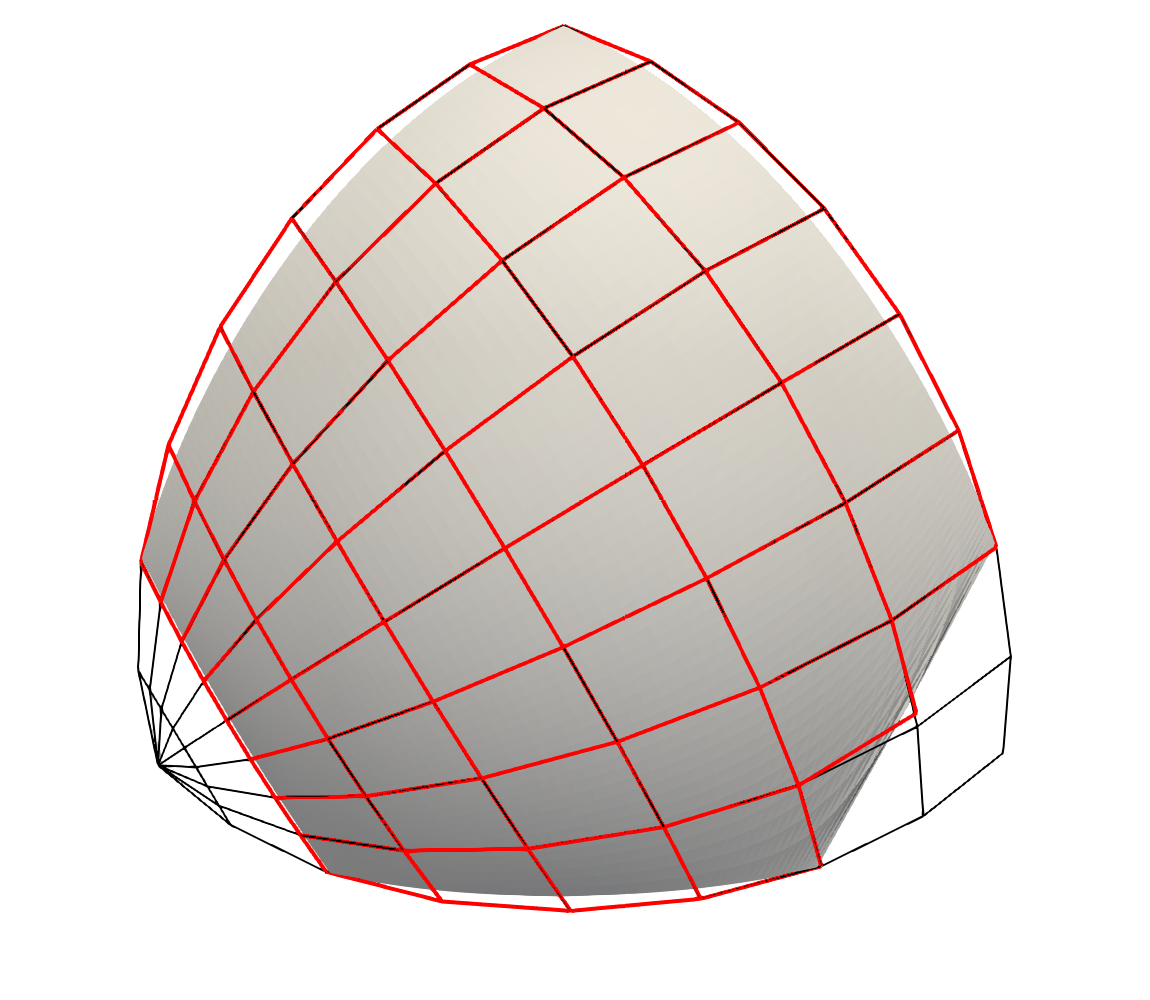
\includegraphics[height=.35\textheight]{images/warren-quad.png}
  \end{columns}
\end{frame}

\subsection{Kato's patch}

\begin{frame}
  \frametitle{Kato's patch}
  \begin{columns}
    \column{0.65\textwidth}
    \begin{itemize}
    \item Transfinite surface interpolation
    \item Blended sum of \emph{ribbons}
    \item $(s_i,h_i)$ parameters for each ribbon
      \[ s_i := h_{i-1} / (h_{i-1} + h_{i+1}) \]
    \item Simple $G^2$ continuity
    \item Singular blending function
      \begin{itemize}
      \item $0/0$ at the corners
      \end{itemize}
    \item High rational degree
      \begin{itemize}
      \item Because of rational $s_i$
      \end{itemize}
    \end{itemize}
    \column{0.35\textwidth}
    \centering
    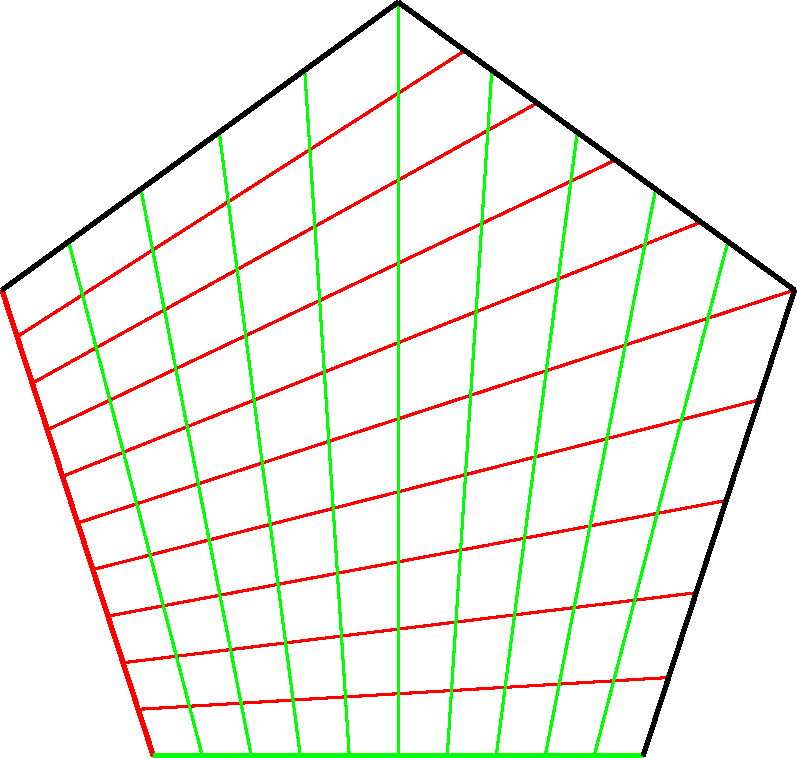
\includegraphics[width=.9\textwidth]{images/s-params.pdf}\\
    {\tiny $s_i$ isolines}\\
    \vspace{1em}
    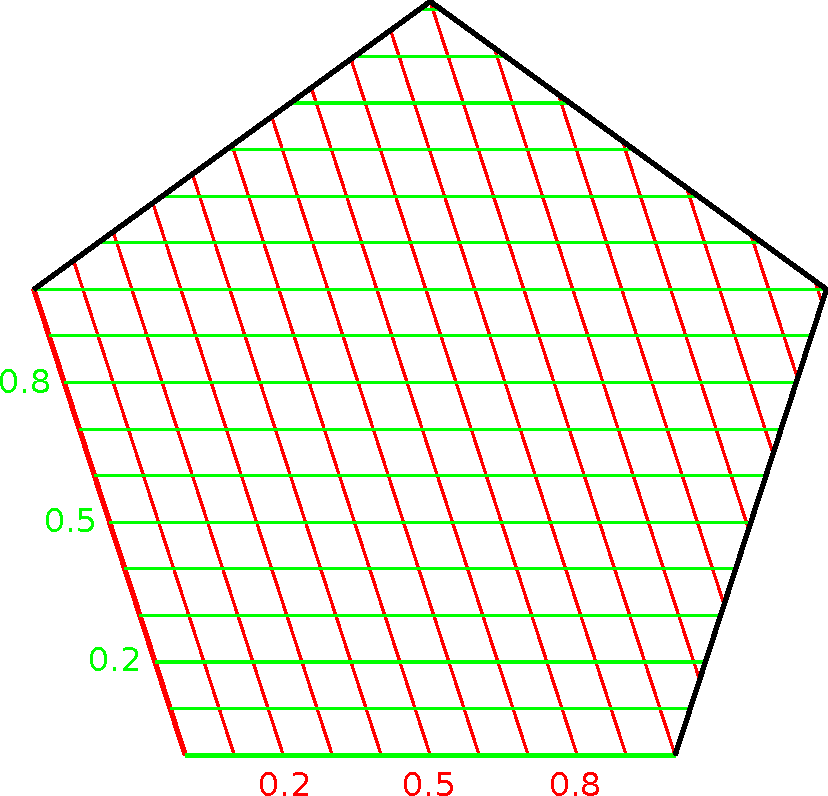
\includegraphics[width=.9\textwidth]{images/h-params.pdf}\\
    {\tiny $h_i$ isolines}\\
  \end{columns}
\end{frame}

\subsection{Charrot--Gregory patch}

\begin{frame}
  \frametitle{Charrot--Gregory patch}
  \begin{columns}
    \column{0.6\textwidth}
    \begin{itemize}
    \item Transfinite surface interpolation
    \item Blended sum of corner interpolants
      \begin{itemize}
      \item Can be reformulated to ribbons
      \end{itemize}
    \item Radial parameterization
      \begin{itemize}
      \item Same as $s_i$ parameters
      \end{itemize}
    \end{itemize}
    \vfill
    \begin{block}{Special case for $n=3$}
      \begin{itemize}
      \item Parameterization with $h_i$
      \item Much lower degree
      \end{itemize}
    \end{block}
    \column{0.4\textwidth}
    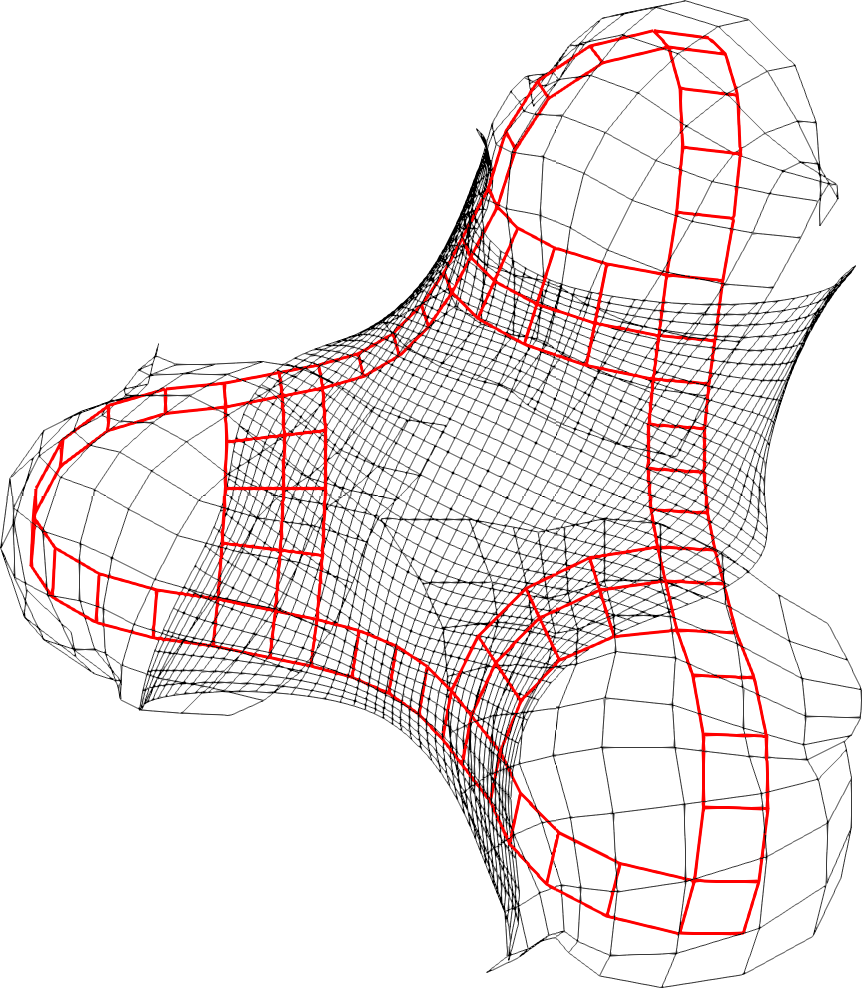
\includegraphics[width=\textwidth]{images/trebol3-cnet.png}
  \end{columns}
\end{frame}

\section{Singularities}

\begin{frame}
  \frametitle{Control net quality}
  \begin{columns}
    \column{0.6\textwidth}
    \begin{itemize}
    \item Control points become erratic\\near singularities
      \begin{itemize}
      \item S-patch: dashed circle ($n>3$)
      \item Warren's patch: always ($n>3$)
      \item Kato's patch: always
      \item Charrot-Gregory patch: red lines
      \end{itemize}
    \item More sides, more problems
    \item Rotation may help with $n=5,6$
    \end{itemize}
    \column{0.4\textwidth}
    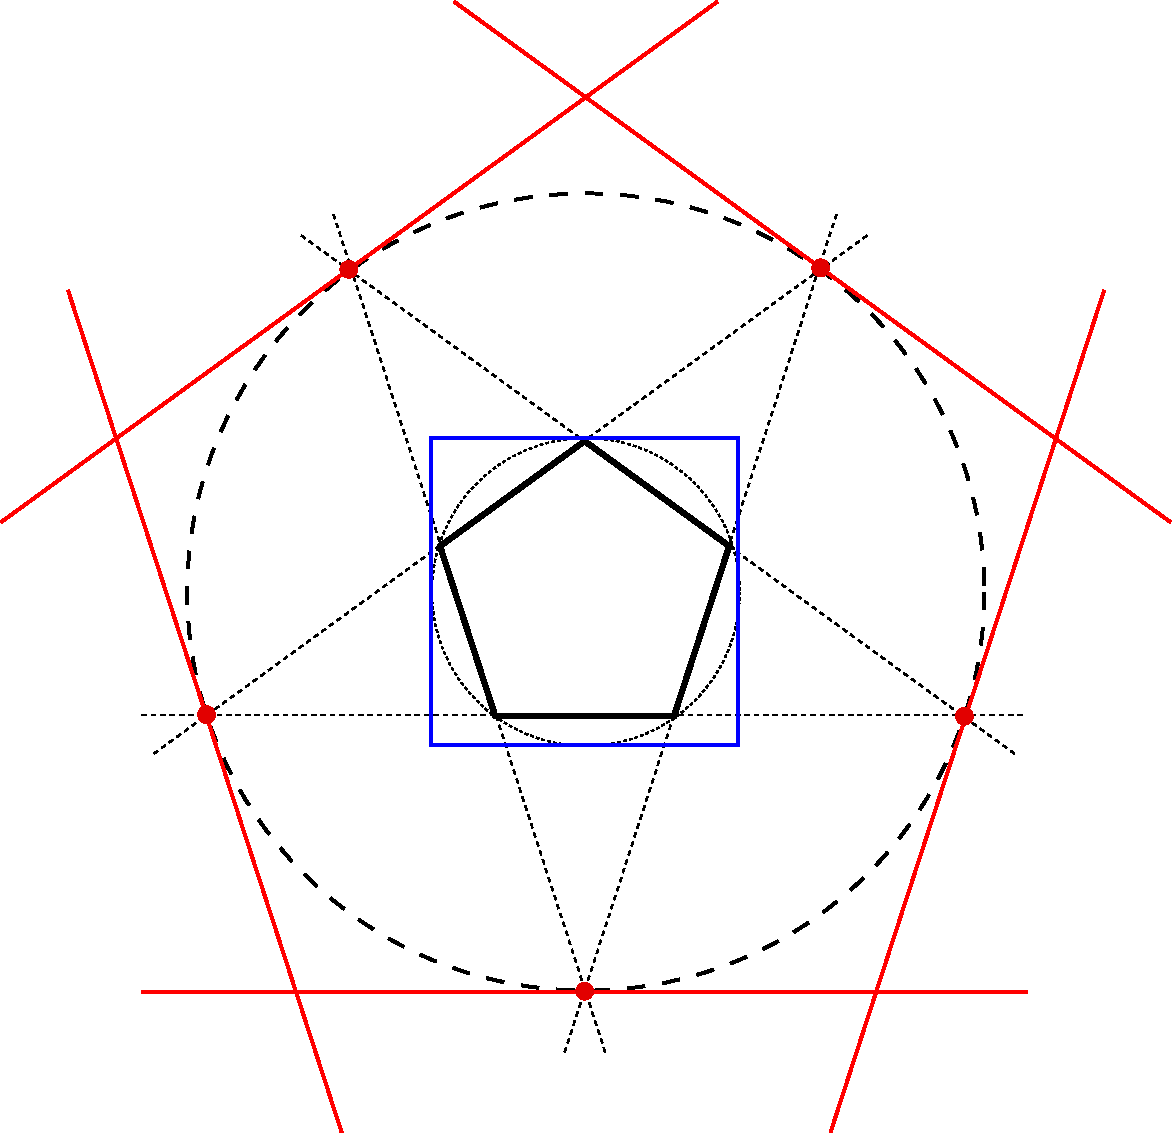
\includegraphics[width=\textwidth]{images/singularities.pdf}
  \end{columns}
  \vfill
  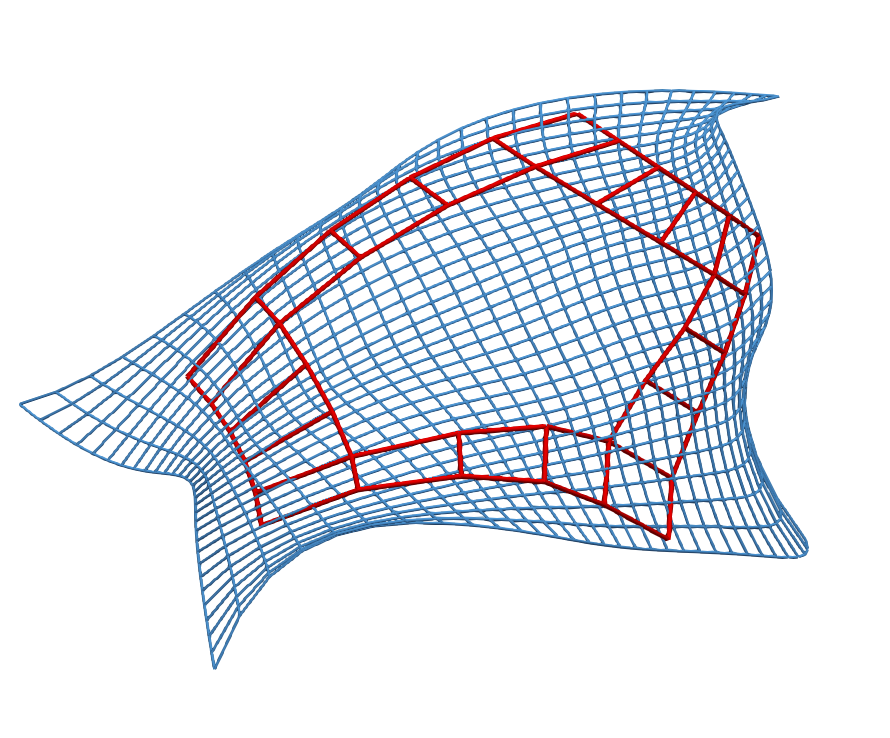
\includegraphics[width=.32\textwidth]{images/rotations/40.png}
  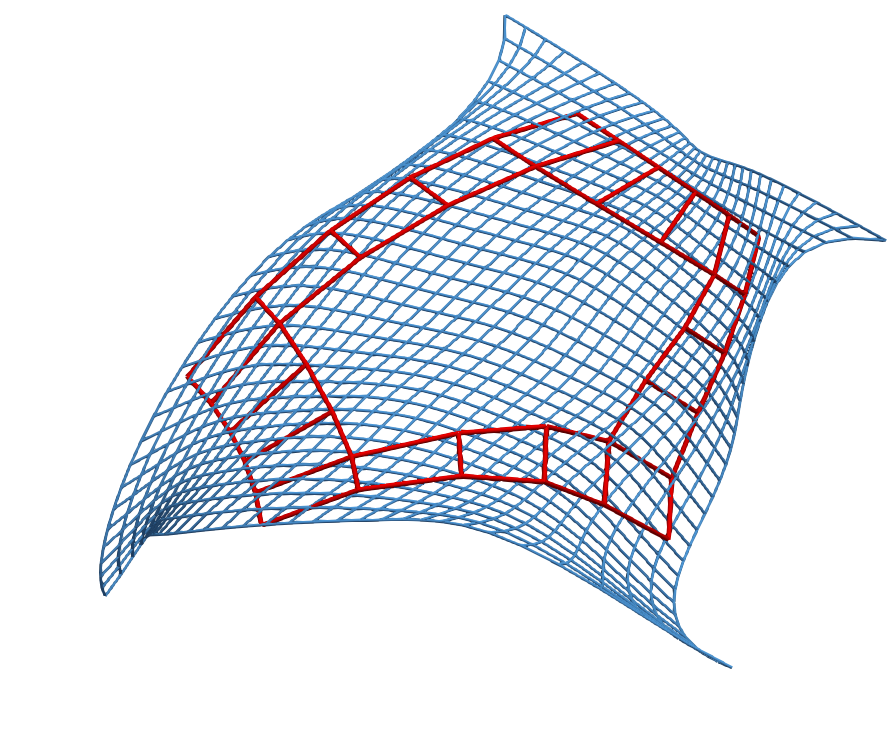
\includegraphics[width=.32\textwidth]{images/rotations/75-optimal.png}
  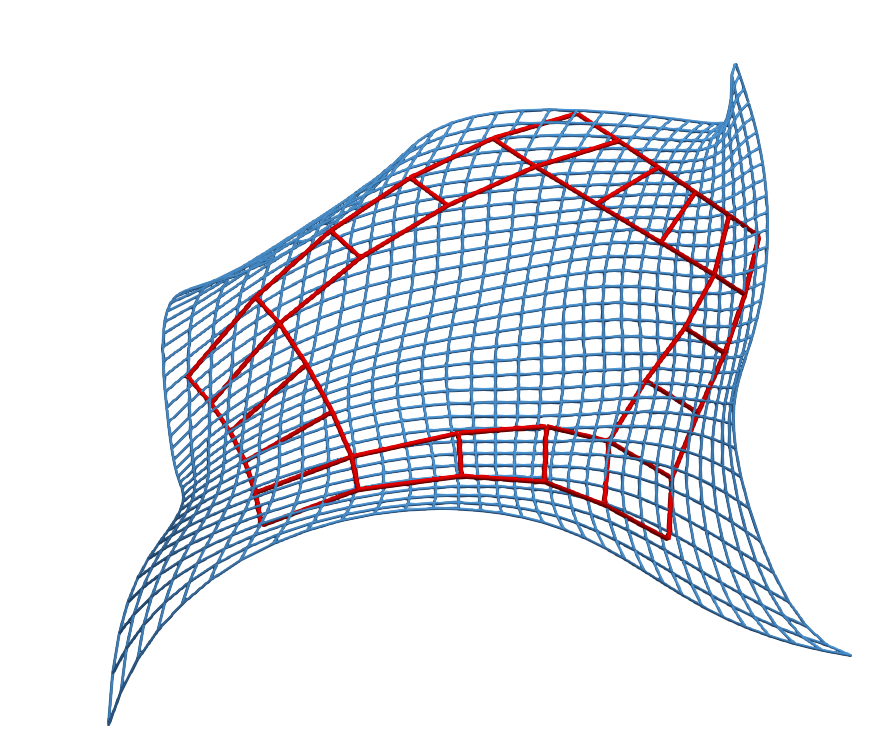
\includegraphics[width=.32\textwidth]{images/rotations/20.png}
\end{frame}

\begin{frame}
  \frametitle{Using a larger $n$-sided domain}
  \begin{columns}
    \column{0.6\textwidth}
    \begin{itemize}
    \item Blue rectangle: $[0,1]\times[0,1]$\\relative to default domain
    \item Green rectangle: $[0,1]\times[0,1]$\\relative to enlarged domain
    \item Trimming curves outside $[0,1]^2$
    \item Not standard
      \begin{itemize}
      \item May or may not be supported
      \item Rhinoceros\textsuperscript\textregistered\ 3D: partial support
      \end{itemize}
    \end{itemize}
    \column{0.4\textwidth}
    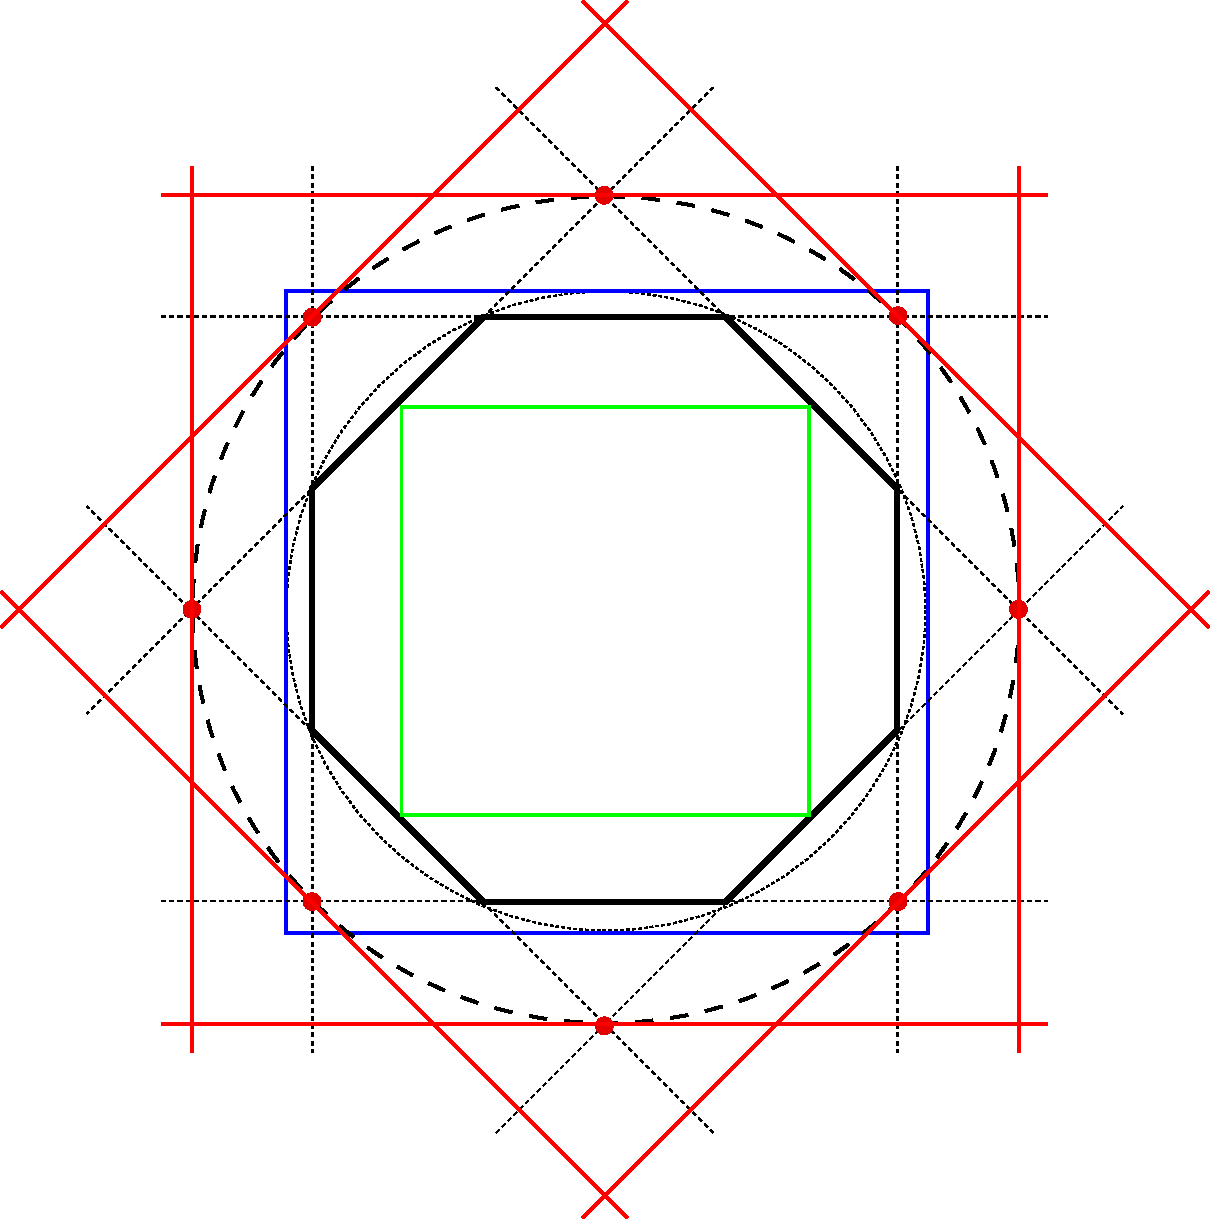
\includegraphics[width=\textwidth]{images/singularities2.pdf}
  \end{columns}
  \vfill
  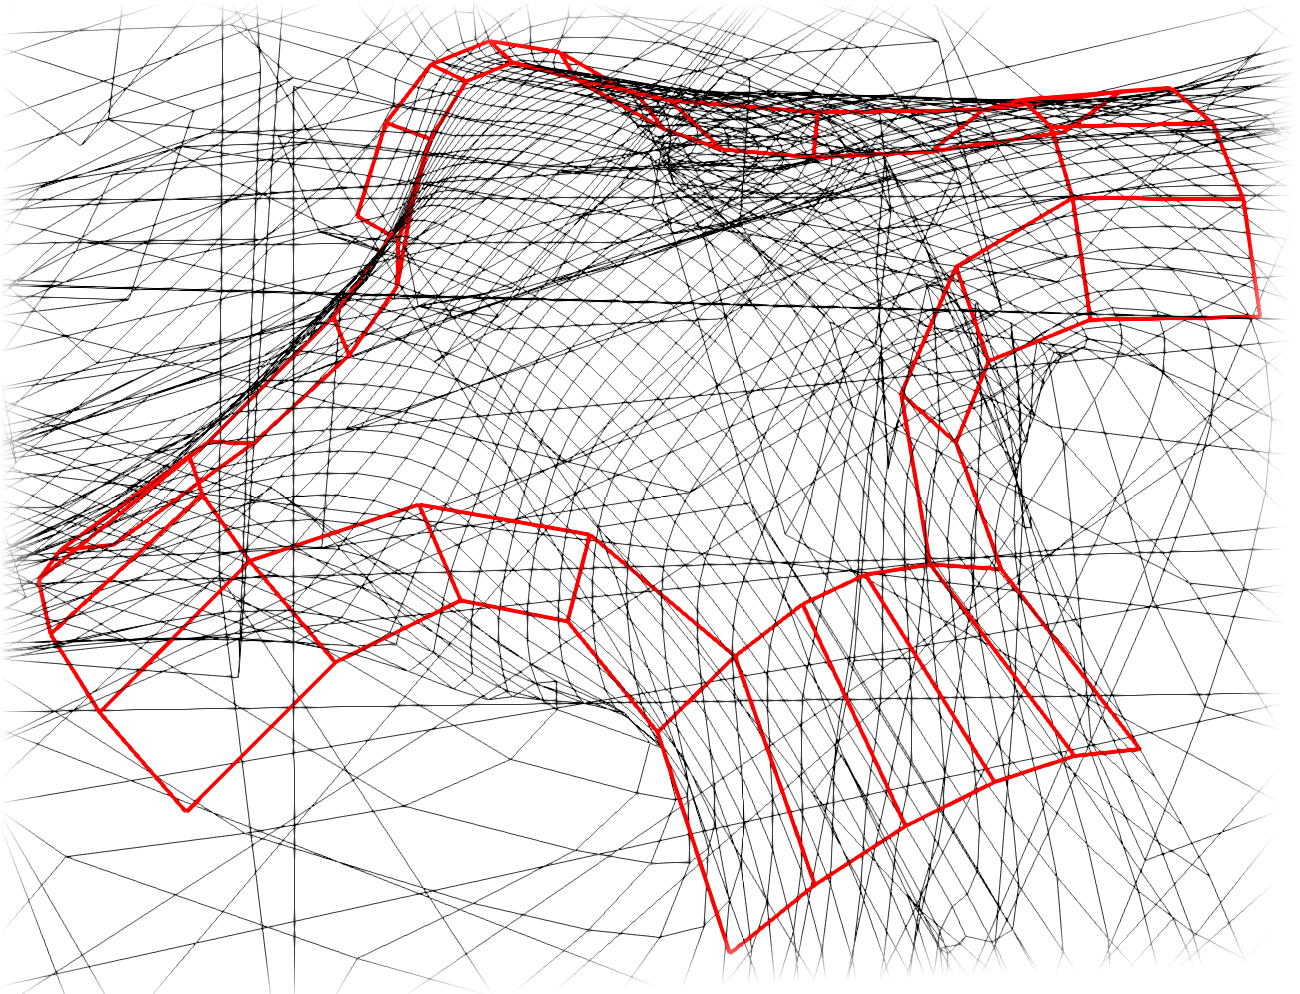
\includegraphics[width=.33\textwidth]{images/8sided-1.png}
  \hfill
  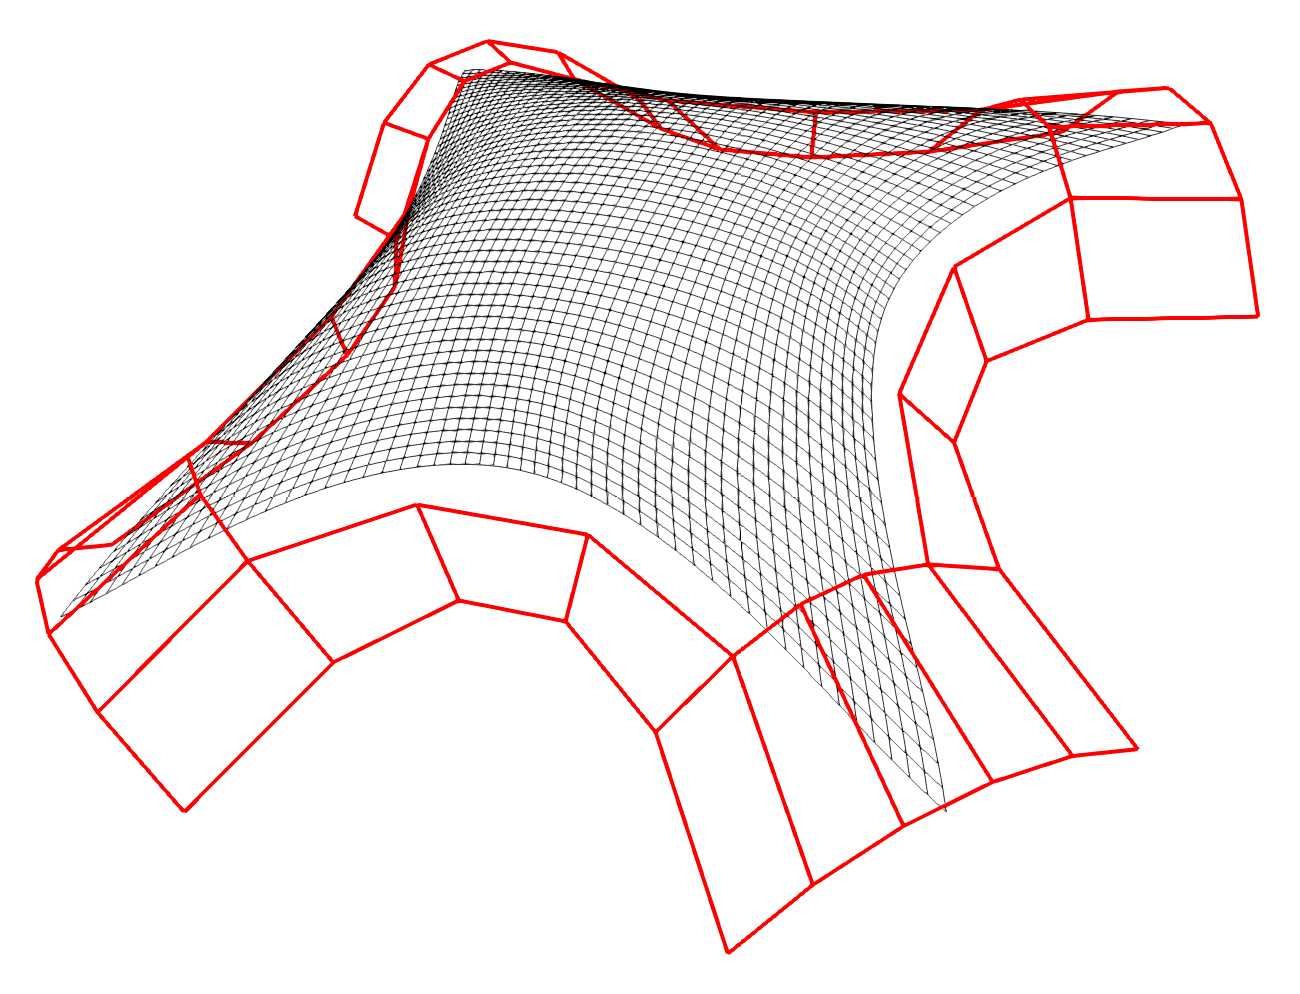
\includegraphics[width=.33\textwidth]{images/8sided-2.png}
  \hfill
  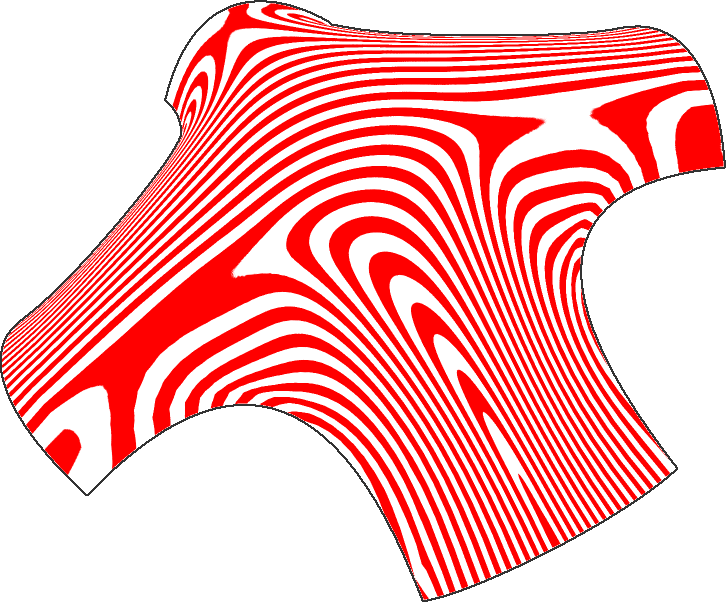
\includegraphics[width=.29\textwidth]{images/8sided-3.png}
\end{frame}

\section{Test results}

\begin{frame}
  \frametitle{Examples in Rhinoceros\textsuperscript\textregistered\ 3D}
  \parbox{.45\textwidth}{
    \centering
    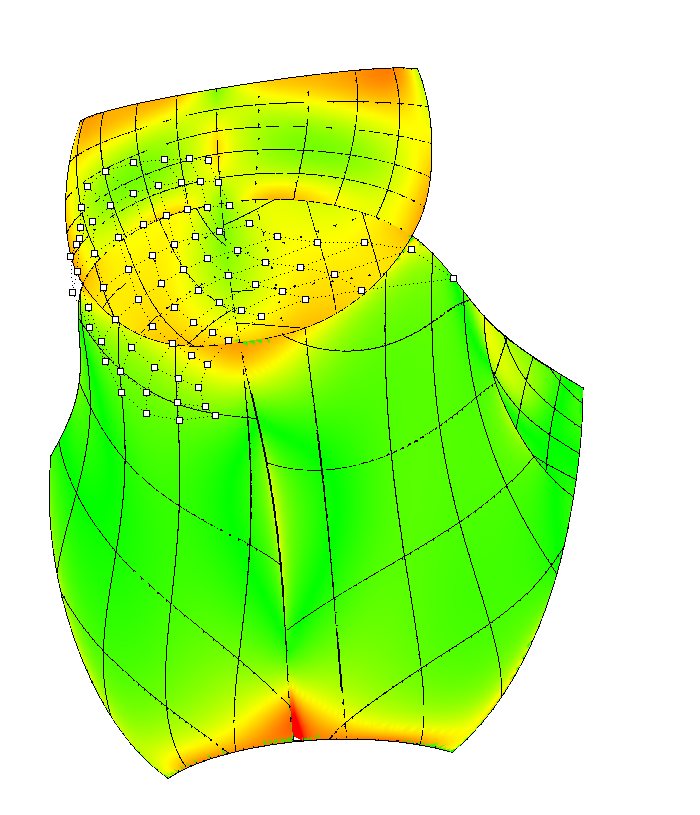
\includegraphics[width=.45\textwidth]{images/cagd86/spatch3.png}\\
    S-patch
  }
  \hfill
  \parbox{.45\textwidth}{
    \centering
    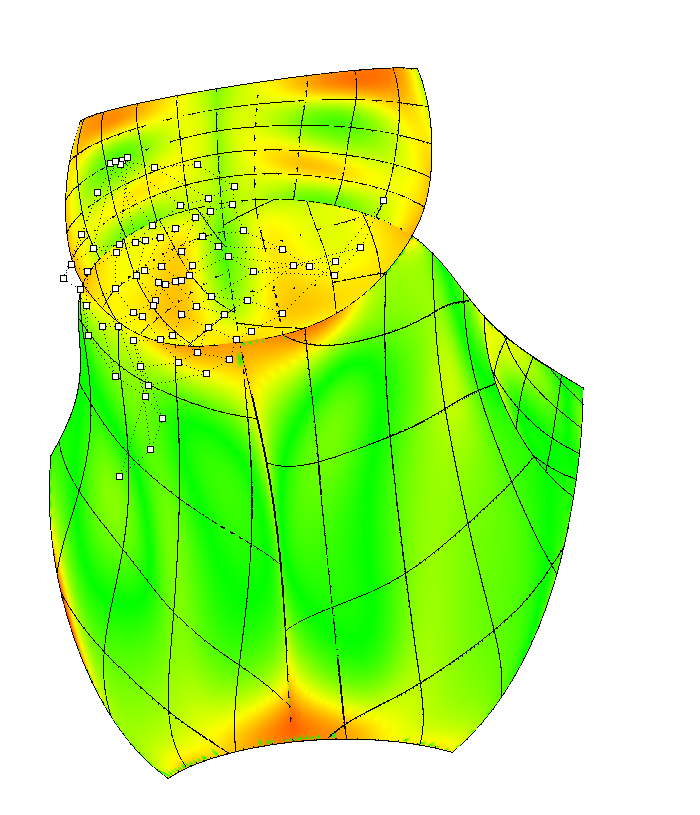
\includegraphics[width=.45\textwidth]{images/cagd86/cg3.png}\\
    Charrot--Gregory patch
  }
\end{frame}

\begin{frame}
  \frametitle{Examples in Rhinoceros\textsuperscript\textregistered\ 3D}
  \parbox{.45\textwidth}{
    \centering
    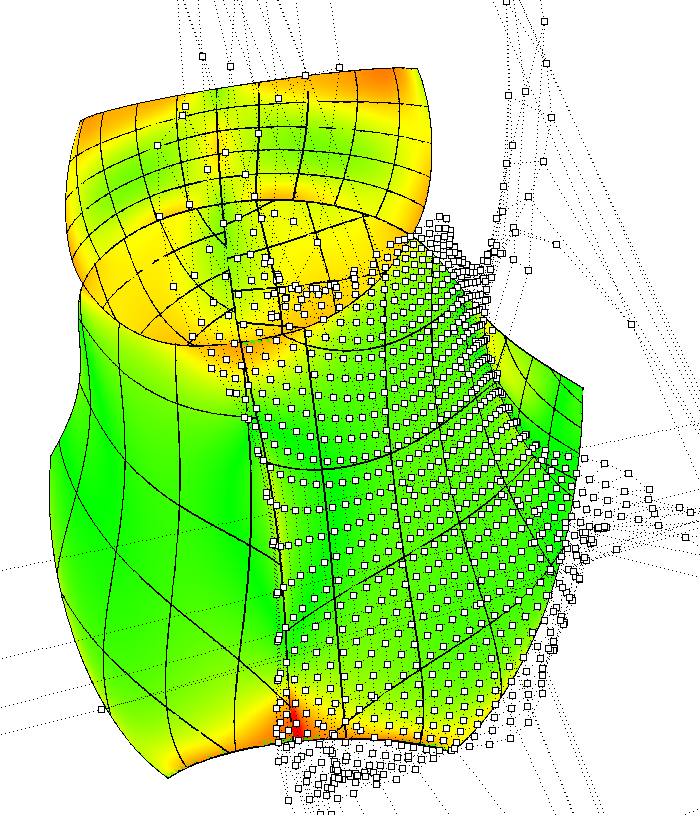
\includegraphics[width=.45\textwidth]{images/cagd86/spatch1.png}\\
    S-patch
  }
  \hfill
  \parbox{.45\textwidth}{
    \centering
    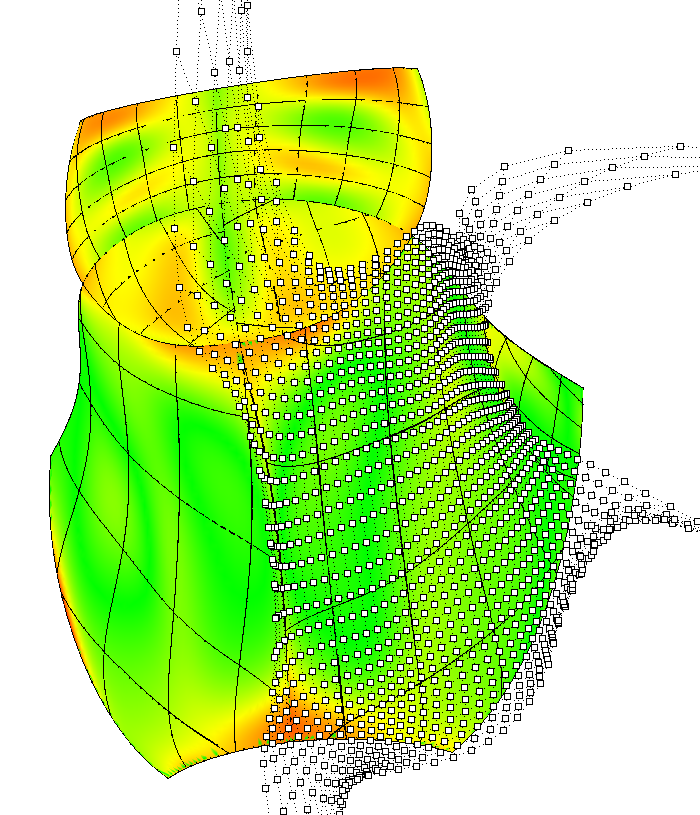
\includegraphics[width=.45\textwidth]{images/cagd86/cg1.png}\\
    Charrot--Gregory patch
  }
\end{frame}

\begin{frame}
  \frametitle{Examples in Rhinoceros\textsuperscript\textregistered\ 3D}
  \parbox{.45\textwidth}{
    \centering
    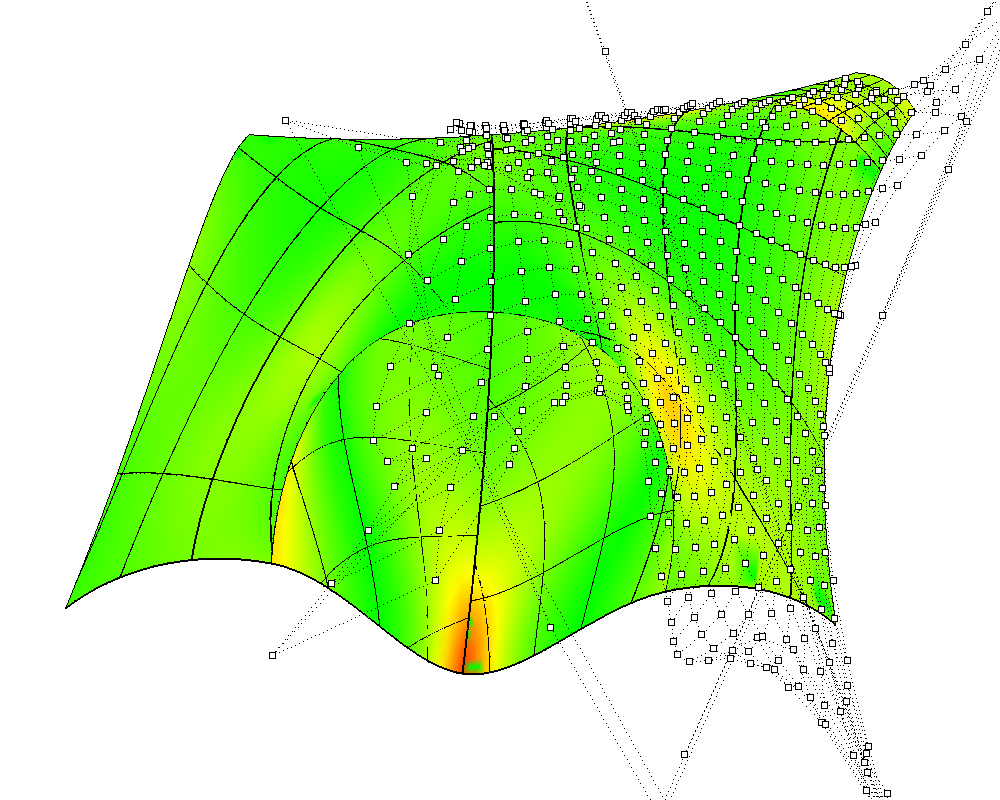
\includegraphics[width=.47\textwidth]{images/pocket/spatch1.png}\\
    S-patch
  }
  \hfill
  \parbox{.45\textwidth}{
    \centering
    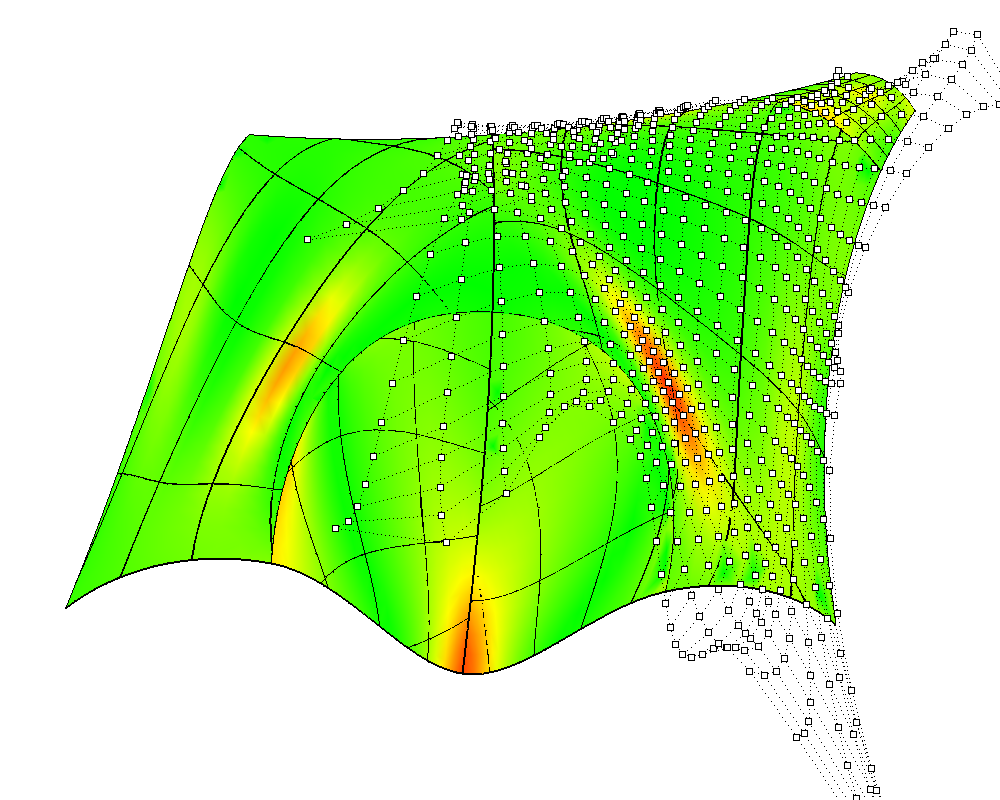
\includegraphics[width=.47\textwidth]{images/pocket/cg1.png}\\
    Charrot--Gregory patch
  }
\end{frame}

\begin{frame}
  \frametitle{Examples in Rhinoceros\textsuperscript\textregistered\ 3D}
  \parbox{.45\textwidth}{
    \centering
    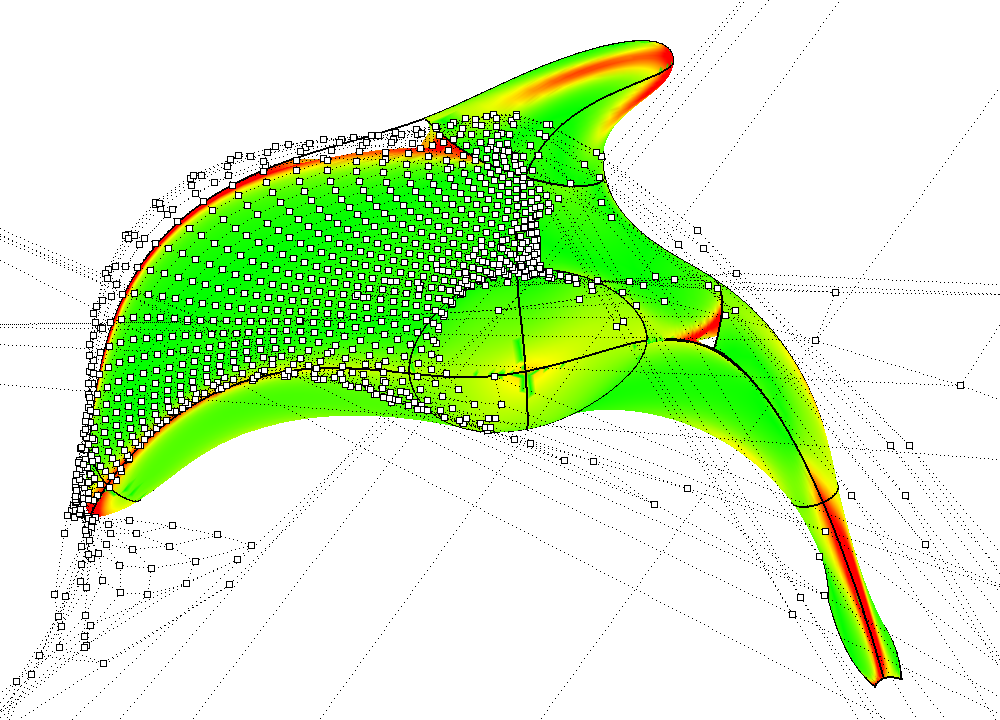
\includegraphics[width=.49\textwidth]{images/dolphin/spatch1.png}\\
    S-patch
  }
  \hfill
  \parbox{.45\textwidth}{
    \centering
    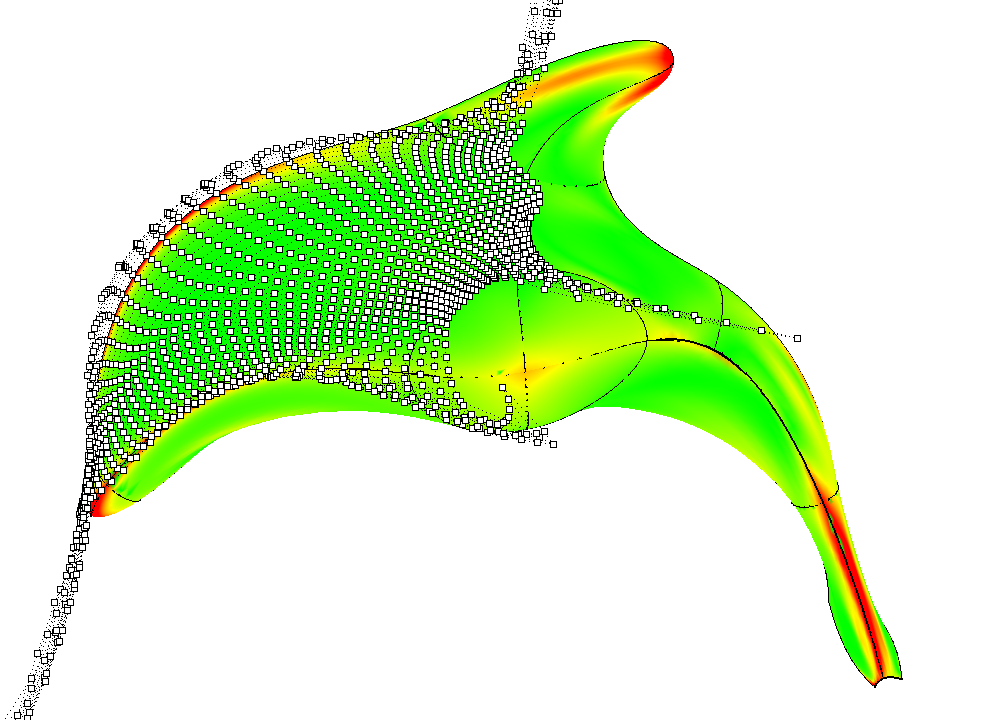
\includegraphics[width=.49\textwidth]{images/dolphin/cg1.png}\\
    Charrot--Gregory patch
  }
\end{frame}

\section {Conclusions}

\begin{frame}
  \frametitle{Conclusions}
  \begin{table}
    \centering
    \small
    \begin{tabular}{c|c|c|c|c}
      $n$ & S-patch & Warren & Kato & Charrot--Gregory \\ \hline
      3 & \multicolumn{2}{c|}{$d[+3]$ (both B\'ezier triangles)} & \cellcolor{light-gray}$3d+5$ & $d+3$ \\ \hline
      5 & \cellcolor{light-light-gray}$3d[+9]$ & $\approx 3d$ & \cellcolor{light-gray}$5d+9$ & $5d+6$ \\ \hline
      6 & \cellcolor{light-light-gray}$4d[+12]$ & $3d$ & \cellcolor{light-gray}$6d+11$ & $6d+8$ \\ \hline
      7+ & \cellcolor{light-gray}$(n-2)(d[+3])$ & $\qquad$N/A$\qquad$ & \cellcolor{light-gray}$nd+2n-1$ & \cellcolor{light-gray}$nd+2n-4$ \\ \hline
    \end{tabular}
    \caption{Rational degrees (grey cells: singularity problems)}
  \end{table}
  \vfill
  \begin{itemize}
  \item Fast \& simple conversion based on implicit line equations
  \item Comparison of four natively multi-sided representations
  \item Control net quality \& singularity problems
  \item Solution using larger multi-sided domains
  \end{itemize}
  \vfill
  \centering
  New low-degree scheme with multi-sided shape control?
\end{frame}

\end{document}
